\documentclass[a4paper]{instrumentacao}

\usepackage{listings}
\usepackage{etoolbox}

\newtoggle{attachments}
\togglefalse{attachments}

\graphicspath{
	{../Resources/Images/}
	{../Resources/Mathematica/images/}
	{../Resources/MATLAB/images/}
}

\title{Alguns Efeitos Físicos Explorados em Sensores}
\author{Rogiel Sulzbach \and Rodrigo de Castro Silveira \and Yi Chen Wu}
\startdate{28 de março de 2016}
\finishdate{24 de abril de 2016}
\emails{
	\emailaddress{R.J.S.}{rogiel@rogiel.com},
	\emailaddress{R.C.S.}{csilveira.rodrigo@gmail.com} e
	\emailaddress{Y.C.}{yichenpoa@gmail.com}
}
\resume{Exploração de um sensor potenciométrico utilizado para estimar a curva de posição em função do tempo de um pêndulo, exploração da medida de campo magnético através de um sensor eletrônico de efeito Hall e experimentação do acionamento de um conjunto de 2 \textit{LEDs} utilizando o software LabVIEW.}
\abstract{Exploration of a potentiometric sensor used to estimate the time curve of a pendulum, measurement of a magnetic field using a Hall sensor and experimentation of a trigger system for a group of 2 LEDs using LabVIEW software.}
\keywords{pêndulo; sensor potenciométrico; efeito Hall; LabVIEW.}
\institute{Universidade Federal do Rio Grande do Sul, Departamento de Engenharia Elétrica, Curso de Engenharia Elétrica, Instrumentação A, Profs. Dr. Alexandre Balbinot e Dra. Léia Bagesteiro}

\headertext{Efeitos físicos}

\begin{document}
\maketitle

\todo{arrumar datas}

\chapter{Introdução}
Nesta atividade de laboratório, tem-se objetivo de explorar e entender o funcionamento dos efeitos físicos de dois tipos de sensores. Um sensor potenciométrico e outro de efeito Hall linear.

\chapter{Metodologia Experimental}
\section{Sensor potenciométrico}
Para a atividade do sensor potenciométrico, foi desenvolvido um pêndulo cujo eixo estava conectado a um potenciômetro. A construção está ilustrada na Figura \ref{fig:pendulo}:

\begin{figure}[H]
\centering
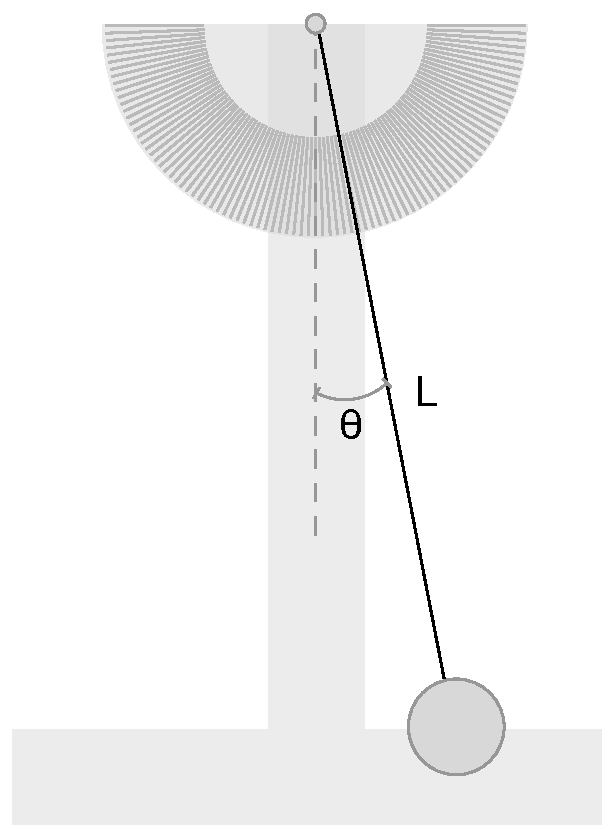
\includegraphics[width=0.4\textwidth]{Pendulo.pdf}
\caption{Estrutura do pêndulo}
\label{fig:pendulo}
\end{figure}
onde $\theta$ é o ângulo de inclinação do pêndulo em relação a origem (linha tracejada) e $L$ é o comprimento do pêndulo. Para este experimento, foi utilizado o comprimento do pêndulo L=27.5cm(centímetro), medido com uma régua da Maped cuja resolução é de 0.1cm.

Este pêndulo pode ser modelado eletricamente pelo circuito da Figura \ref{fig:pendulo-equivalente}:

\begin{figure}[H]
\centering
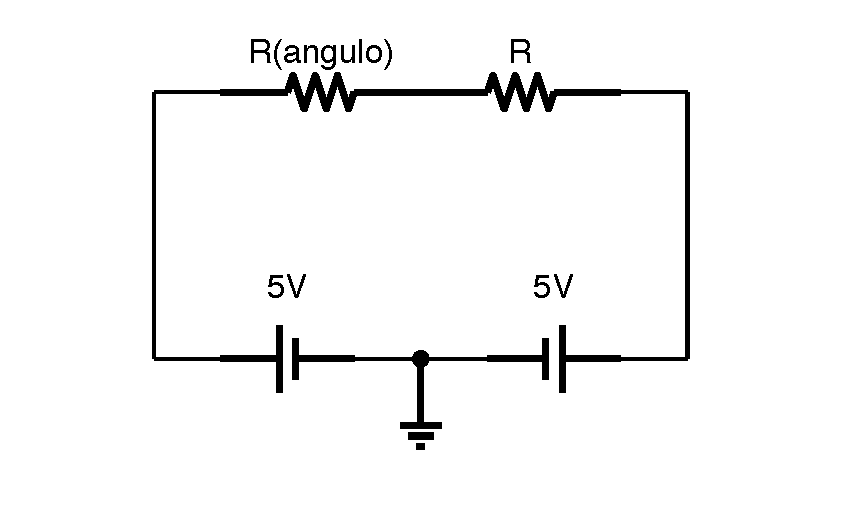
\includegraphics[width=0.6\textwidth]{Pendulo-Circuito.pdf}
\caption{Modelo elétrico do pêndulo}
\label{fig:pendulo-equivalente}
\end{figure}

onde $R(angulo)$ é uma resistência variável em função do ângulo $\theta$.

A fim de extrair a função de transferência do sensor, realiza-se um experimento com repetição onde, através de um voltímetro, mede-se a tensão elétrica sobre o resistor $R(\theta)$ em função do ângulo $\theta$. Com esse experimento, pode-se realizar um \textit{fit} cuja função foi utilizada como a função de transferência do sensor. Uma vez que o potenciômetro é linear, espera-se que a função de transferência é dada na forma da Equação \ref{eq:pendulo-tf-forma} e conforme a estrutura apresentada na Figura \ref{fig:pendulo}:

\begin{equation}
	R(\theta) = R_0 + R_1 \times \theta
	\label{eq:pendulo-tf-forma}
\end{equation}

onde $R(\theta)$ é a resistência elétrica do pêndulo em $\Omega$(ohm, unidade de medida da resistência elétrica) para um dado ângulo de inclinação, $R_0$ é a resistência do pêndulo em $\Omega$ no ângulo de zero graus em relação a origem(a linha tracejada), $R_1$ é a variação de resistência elétrica do pêndulo em $\Omega / rad$ em função da variação de ângulo e $\theta$ é a inclinação do pêndulo em $rad$(radiano) relativa a sua posição de repouso.

Para minimizar o efeito de \textit{ripple} de tensão elétrica da fonte de alimentação, foram utilizados dois reguladores de tensão elétrica, sendo um dele foi LM7805\todo{colocar o fabricante, existem vários, confirmar em cima do CI}, regulador de $(5 \pm 0.2)V$\cite{datasheet-lm7805} e outro foi regulador LM7905 \todo{colocar o fabricante, existem vários, confirmar em cima do CI}, de $(-5 \pm 0.2)V$\cite{datasheet-lm7905}. O mesmo conjunto de reguladores foi utilizado para alimentar todos componentes elétricos externos. De acordo com o fabricante, este regulador possui um tolerância de 0.2V(volt) com uma distribuição uniforme de probabilidade. A incerteza correspondente, $\delta_{regulador}$, pode ser obtida pela Equação \ref{eq:incerteza-regulador}:

\begin{equation}
	\delta_{regulador} = \frac{\Delta_{regulador}}{\sqrt{3}} \approx 0.12 V
	\label{eq:incerteza-regulador}
\end{equation}

\subsection{Modelagem do sistema de aquisição de dados do pêndulo}

Para obter a resposta temporal do pêndulo, foi utilizado um mecanismo de aquisição de dados conforme a Figura \ref{fig:pendulo-fluxo-medidas}:

\begin{figure}[H]
\centering
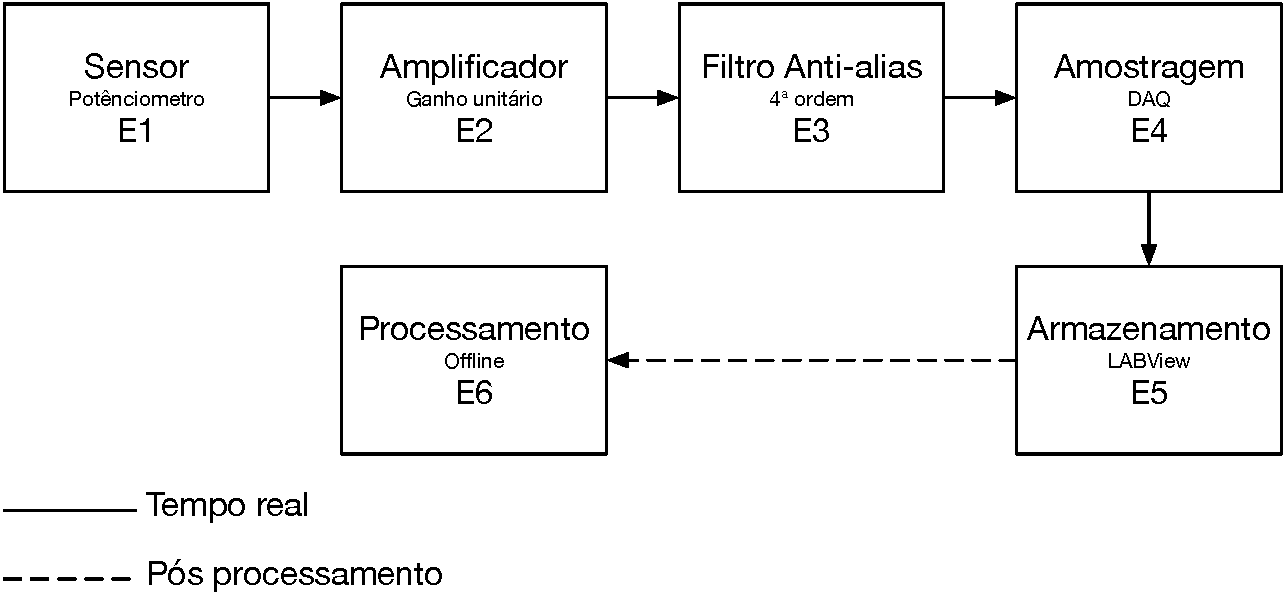
\includegraphics[width=\textwidth]{Pendulo-Fluxograma.pdf}
\caption{Fluxo de aquisição de dados do sistema.}
$E_n$ indica as etapas de aquisição de dados.
\label{fig:pendulo-fluxo-medidas}
\end{figure}

\begin{itemize}
	\item \textbf{E1}: representa o sensor utilizado, no caso deste experimento, foi um potenciômetro;
	\item \textbf{E2}: representa um amplificador com ganho unitário (\textit{buffer});
	\item \textbf{E3}: representa o filtro anti-alias utilizado para o processo de amostragem;
	\item \textbf{E4}: representa o processo de amostragem realizado, utilizando o LabVIEW e o DAQ (Data Acquisition device)
	\item \textbf{E5}: no LabVIEW foram armazenados os dados amostrados;
	\item \textbf{E6}: após do armazenamento dos dados, foi realizado o processamento destes dados.
\end{itemize}

A cadeia de medidas deste experimento pode ser representada pelo diagrama de blocos da Figura \ref{fig:pendulo-cadeia-medidas}:

\begin{figure}[H]
\centering
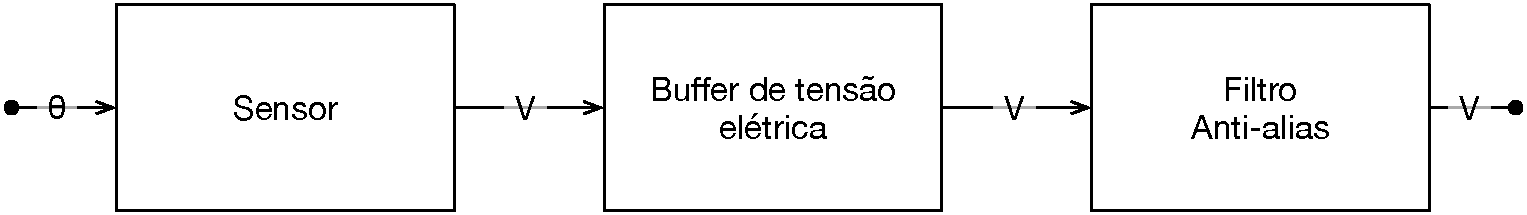
\includegraphics[width=\textwidth]{Cadeia de medida.pdf}
\caption{Cadeia de medida com grandezas de entrada e saída}
\label{fig:pendulo-cadeia-medidas}
\end{figure}

Para a etapa E1, utilizou-se um 

de \todo{qual a resistência dele?} com uma incerteza informada pelo fabricante de 100 $\Omega$ \todo{chute}.

Para a etapa E2, utilizou-se um amplificador operacional LM741\cite{datasheet-lm741} configurado como um seguidor de tensão elétrica, \textit{buffer}, conforme o esquemático elétrico apresentado na Figura \ref{fig:buffer-tensão}:

\begin{figure}[H]
\centering
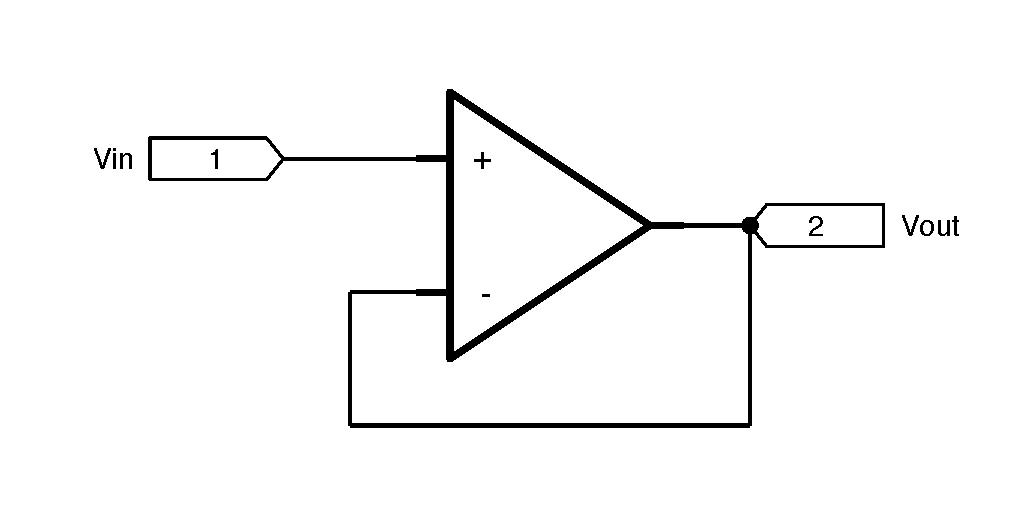
\includegraphics[width=\textwidth]{Buffer-tensao.pdf}
\caption{Circuito elétrico do \textit{buffer} de tensão elétrica}
\label{fig:buffer-tensão}
\end{figure}

\noindent
onde $V_{in}$ é a tensão elétrica de entrada e $V_{out}$ é a tensão elétrica de saída do \textit{buffer}. A função de transferência do \textit{buffer} é dada, trivialmente, pela Equação \ref{eq:buffer}

\begin{equation}
	V_{out} = V_{in}
	\label{eq:buffer}
\end{equation}

Para a etapa E3, utilizou-se um filtro ativo anti-alias do tipo \textit{Butterworth} de quarta ordem com frequência de corte de 100 $Hz$(hertz). Esta decisão foi tomada para que a fase não-linear de um filtro de \textit{Butterworth} não pudesse causar qualquer alteração no sinal amostrado. O filtro foi implementado utilizando a topologia de filtros ativos de \textit{Sallen-Key} e utilizou-se o amplificador operacional LM741 em dois estágios. Cada estágio do filtro é implementado pelo bloco da Figura \ref{fig:filtro-estagio}:

\begin{figure}[H]
\centering
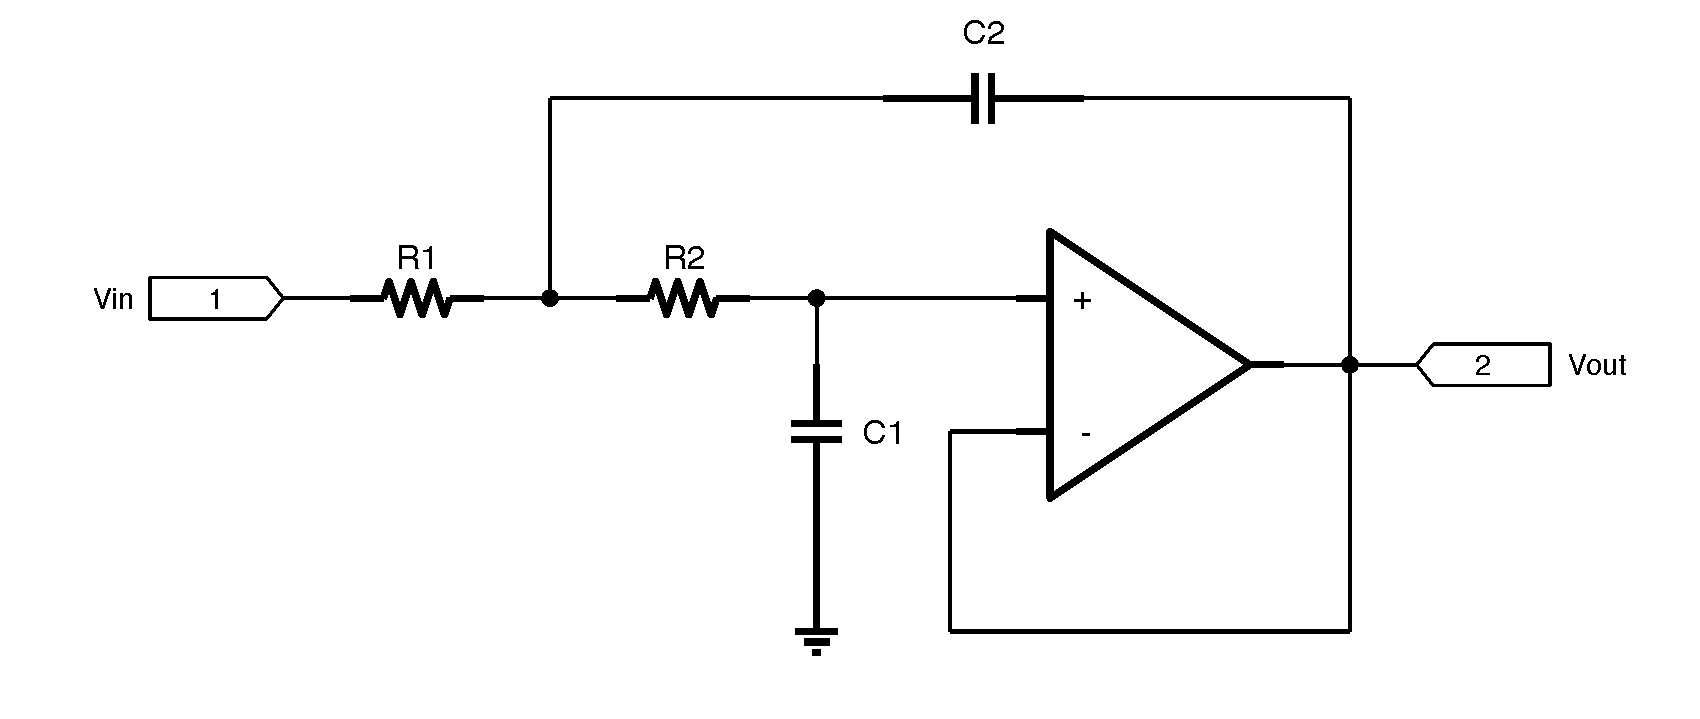
\includegraphics[width=\textwidth]{Filtro-estagio.pdf}
\caption{Esquemático elétrico do \textit{buffer} de tensão elétrica}
\label{fig:filtro-estagio}
\end{figure}

\noindent
onde os resistores $R_1$ e $R_2$ e os capacitores $C_1$ e $C_2$ determinam a frequência de corte do filtro, $V_{in}$ é a tensão elétrica de entrada do estágio do filtro e $V_{out}$ é a tensão elétrica de saída do estágio do filtro.

A função de transferência do estágio no domínio da frequência é dada pela Equação \ref{eq:filtro-tf}:

\begin{equation}
	H_{\text{filtro}, \text{estágio n}}(s) = \frac{1}{C_1 C_2 s^2 \left(\frac{1}{C_2 s}\left(R_1+R_2\right)+\frac{1}{C_1 C_2 s^2}+R_1 R_2\right)}
	\label{eq:filtro-tf}
\end{equation}

A associação dos estágios é dada pela multiplicação das funções de transferência de cada estágio (Equação \ref{eq:filtro-tf}) no domínio frequência, conforme Equação \ref{eq:filtro-tf-assoc}

\begin{equation}
	\frac{V_{in}(s)}{V_{out}(s)} = H_{\text{filtro}, \text{estágio 1}}(s) \times H_{\text{filtro}, \text{estágio 2}}(s)
	\label{eq:filtro-tf-assoc}
\end{equation}

\noindent
onde a função de transferência resultante é dada pela Equação \ref{eq:filtro-tf-completa}:

\begin{equation}
	\small
	\frac{V_{out}}{V_{in}} = \frac{1}{\left(C_1 C_2 R_1 R_2 s^2+C_1 R_1 s+C_1 R_2 s+1\right) \left(C_3 C_4 R_3 R_4
   s^2+C_3 R_3 s+C_3 R_4 s+1\right)}
	\label{eq:filtro-tf-completa}
\end{equation}

Os pólos da função de transferência da Equação \ref{eq:filtro-tf-completa}, estão definidos como as frequências das Equações \ref{eq:filtro-tf-polo1}, \ref{eq:filtro-tf-polo2}, \ref{eq:filtro-tf-polo3} e \ref{eq:filtro-tf-polo4}:

\begin{eqnarray}
	p_{1} &=& \frac{-\sqrt{\left(C_1 R_1+C_1 R_2\right){}^2-4 C_1 C_2 R_1 R_2}-C_1 R_1-C_1 R_2}{2 C_1 C_2 R_1 R_2} \label{eq:filtro-tf-polo1} \\
	p_{2} &=& \frac{\sqrt{\left(C_1 R_1+C_1 R_2\right){}^2-4 C_1 C_2 R_1 R_2}-C_1 R_1-C_1 R_2}{2 C_1 C_2 R_1 R_2} \label{eq:filtro-tf-polo2} \\
	p_{3} &=& \frac{-\sqrt{\left(C_3 R_3+C_3 R_4\right){}^2-4 C_3 C_4 R_3 R_4}-C_3 R_3-C_3 R_4}{2 C_3 C_4 R_3 R_4} \label{eq:filtro-tf-polo3} \\
	p_{4} &=& \frac{\sqrt{\left(C_3 R_3+C_3 R_4\right){}^2-4 C_3 C_4 R_3 R_4}-C_3 R_3-C_3 R_4}{2 C_3 C_4 R_3 R_4}\label{eq:filtro-tf-polo4} 
\end{eqnarray}

\noindent
onde $p_1$, $p_2$, $p_3$ e $p_4$ são os pólos da função da transferência ideal do filtro.

Resolvendo as Equações \ref{eq:filtro-tf-polo1}, \ref{eq:filtro-tf-polo2}, \ref{eq:filtro-tf-polo3} e \ref{eq:filtro-tf-polo4} para a frequência de 100 $Hz$, uma possível solução para os valores dos resistores($R_1$ e $R_2$) e capacitores($C_1$ e $C_2$) utilizando valores comerciais é dada pela Tabela \ref{tab:filtro-valores}:

\begin{table}[H]
\centering
\caption{Tabela com o valor dos componentes passivos do filtro}
\begin{tabular}{|l|l|l|}
 \hline
 \textbf{Componente} & \textbf{Valor} & \textbf{Tolerância} \\ \hline
 
 $R_1$ & 12 $k\Omega$ 	& 10\% \\ \hline
 $R_2$ & 18 $k\Omega$ 	& 10\% \\ \hline
 $R_3$ & 3.9 $k\Omega$ 	& 10\% \\ \hline
 $R_4$ & 8.2 $k\Omega$ 	& 10\% \\ \hline
 
 $C_1$ & 100 $nF$ 		& 5\% \\ \hline
 $C_2$ & 120 $nF$ 		& 5\% \\ \hline
 $C_3$ & 100 $nF$ 		& 5\% \\ \hline
 $C_4$ & 820 $nF$ 		& 5\% \\ \hline
  
\end{tabular}
\label{tab:filtro-valores}
\end{table}

Com os componentes cujos valores indicados na Tabela \ref{tab:filtro-valores}, a frequência de corte efetiva do filtro é de 98 $Hz$, muito próximo da frequência de 100 $Hz$, que é a frequência desejada para este filtro ativo. A determinação da incerteza propagada dos componentes passivos para a frequência do filtro pode ser obtida utilizando a regra de propagação pela série de Taylor expressa pela Equação \ref{eq:incerteza-propagada}:

\begin{equation}
	\delta_f = \sqrt{
		\sum_{k} 
			\left(\frac{\partial f}{\partial k}\times \delta_k \right)^2
	}
	\label{eq:incerteza-propagada}
\end{equation}

\noindent
onde $f$ é a função de medição, $\delta_f$ é a incerteza propagada para $f$, $k$ são as variáveis com incertezas definidas e $\delta_k$ são as incertezas para cada variável $k$.

\todo{referenciar o script do mathematica}

Com o \textit{software} Wolfram Mathematica, é fácil aproximar a incerteza propagada dos valores dos componentes adicionados ao filtro para a frequência de corte real do filtro. Nas Equações \ref{eq:incerteza-polo-1} e \ref{eq:incerteza-polo-2}, estão indicadas as incertezas propagadas da frequência de corte para cada um dos pólos do filtro. Neste cálculo, as incertezas de parâmetros do amplificador operacional foram desconsideradas para simplificar os cálculos.

\begin{eqnarray}
	f_{1,2} = 98 \pm 20 \label{eq:incerteza-polo-1} \text{ Hz} \\
	f_{3,4} = 98 \pm 27 \label{eq:incerteza-polo-2} \text{ Hz} 
\end{eqnarray}

\noindent
onde $f_{1,2}$ é a frequência de corte para os pólos 1 e 2 e $f_{3,4}$ é a frequência de corte para os pólos 3 e 4.

Logo, através da análise anterior, pode-se concluir que, mesmo no pior caso de incerteza dos componentes, o filtro ainda não será o fator que cause influência no valor amostrado.

Para o processo de amostragem E4, o DAQ USB-6009 da \textit{National Instruments} foi utilizado para levantar os dados experimentais. A entrada lógica deste dispositivo possui 14 \textit{bits} e uma taxa de amostragem de 48 $kS/s$ e possui uma resolução de tensão elétrica na entrada analógica de $1.53 mV$.

\subsection{Levantamento da função de transferência do pêndulo}

Para poder estimar o valor do ângulo de inclinação do pêndulo, em função da tensão elétrica medida pelo fluxo de medida, que foi mostrado na Figura \ref{fig:pendulo-fluxo-medidas}, e, utilizando as funções de transferência definidas para cada um dos blocos, pode-se realizar a extração da função de transferência experimental do pêndulo.

A função de transferência para o sensor já foi obtida no experimento anterior e é dada na equação \ref{eq:pendulo-tf-forma}. Contudo, para utilizá-la nas medidas realizadas, é preciso que a função de transferência inversa seja obtida, conforme a Equação \ref{eq:pendulo-tf-forma-inversa}

\begin{equation}
	\theta = V^{-1}(\theta) = \theta_0 + \theta_1 \times V
	\label{eq:pendulo-tf-forma-inversa}
\end{equation}

onde $\theta$ é a inclinação do pêndulo em radianos, $V^{-1}(\theta)$ é a inversa da função de transferência do pêndulo modelada anteriormente, $\theta_0$ é o \textit{offset} de ângulo correspondente ao \textit{offset} inicial de tensão elétrica e $\theta_1$ é a constante que define a variação de inclinação em função de uma variação de tensão elétrica do sensor.

Para que seja possível comparar os resultados obtidos com e sem o circuito condicionador, é imprescindível que sejam extraídas as funções de transferências equivalentes do pêndulo nas duas situações.

Para extrair a função de transferência experimental do pêndulo sem condicionamento, foi utilizado um multímetro digital Minipa ET-2082B com as especificações de precisão informadas pelo fabricante apresentada na Tabela \ref{tab:precisão-multimetro}. A coluna da precisão é apresentada na forma: $\pm$ (a$\%$ leitura + b dígitos), garantido por 1 ano. Como equipamento já tem mais de um ano de uso sem calibragem, esses dados não são totalmente fidedígnos.


\begin{table}[H]
\centering
\caption{Especificações de precisão do multímetro Minipa ET-2082B para a medição de Tensão DC}
\label{tab:precisão-multimetro}
\begin{tabular}{|c|c|c|}
\hline
\textbf{Faixa} & \textbf{Precisão} & \textbf{Resolução} \\ \hline
200 mV         & \multirow{4}{*}{$\pm$ (0.5\% + 3D)} & 100 $\mu$V \\ \cline{1-1} \cline{3-3} 
2 V            &                              & 1 mV               \\ \cline{1-1} \cline{3-3} 
20 V           &                              & 10 mV              \\ \cline{1-1} \cline{3-3} 
200 V          &                              & 100 mV             \\ \hline
1000 V         & $\pm$ (1.0\% + 5D)           & 1 V                \\ \hline
\end{tabular}
\end{table}

Foi medida a tensão elétrica sobre um dos resistores intermediários do modelo elétrico do pêndulo conforme a Figura \ref{fig:pendulo-equivalente} onde o pêndulo foi alimentado com uma tensão elétrica simétrica de -5V e +5V. Foram feitas medidas em intervalos de 10 em 10 graus de -90 a +90 graus com duas repetições cada medição.

\label{sec:pendulo-calibracao-condicionado}

Para extrair a função de transferência experimental do pêndulo com todo circuito de condicionamento acoplado a ele, foi utilizado um simples programa no LabVIEW que extrai 500 amostras do sinal a uma frequência de 1 $kHz$ e calcula-se a média destes valores. O valor da média das 500 amostras foi utilizado como uma única medida. Assumindo que o ruído gerado pelo conversor analógico-digital ou outra parte do circuito condicionador seja ruído Gaussiano aditivo branco (AWGN) com média zero, logo, a variável estocástica de ruído produzida pelo condicionamento será minimizada.

Com o pêndulo alimentado na mesma forma do experimento sem condicionamento, o dispositivo DAQ foi configurado com entradas digitais diferenciais com o terminal negativo conectado ao terra analógico do regulador de tensão elétrica e o terminal positivo conectado ao pino intermediário do potenciômetro do pêndulo.

Conforme o experimento sem condicionamento, o experimento realizado foi fatorial completo com um fator controlável a 19 níveis (de -90 a +90 graus) com duas repetições por célula.

Após a realização das medidas sem e com condicionamento, foi feito um ajuste de curvas no \textit{software} Wolfram Mathematica para obter a função de transferência experimental para cada um dos experimentos que deve ser dada na forma da Equação \ref{eq:pendulo-tf-forma-inversa}.

\subsection{Curva temporal do pêndulo}

Para extrair a curva temporal do pêndulo, foi utilizada uma configuração igual à do experimento de calibração (página \pageref{sec:pendulo-calibracao-condicionado}) onde o programa do LabVIEW utilizado realizava a aquisição dos dados experimentais de forma temporal a uma taxa de amostragem de 250 $Hz$ com 2000 amostras, totalizando 8 segundos de aquisição de dados.

O formato da onda foi exportado em formato TSV (\textit{tab separated values}) que pode ser importado diretamente no MATLAB, no Wolfram Mathematica ou no LabVIEW posterior à aquisição para processamento dos dados. O formato escolhido foi feito pela facilidade de importação em praticamente qualquer programa que possa manipular os dados. Não foi adicionada nenhuma \textit{header} ao arquivo.

Após a aquisição dos dados, o script do MATLAB localizado na página \todo{referenciar o script}, foi executado para gerar os gráficos e realizar a transformada de Fourier do sinal adquirido.

\section{Efeitos Físicos Utilizados em Sensores}

\subsection{Sensor de Efeito Hall}
Neste experimento foi feita a interface com um módulo sensor de \textit{Efeito Hall Linear}, apresentado na Figura \ref{fig:efeito-hall}, com a Placa DAQ disponibilizada em laboratório.

\begin{figure}[H]
\centering
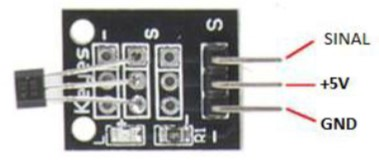
\includegraphics[width=0.3\textwidth]{Imagens/Sensor_Hall.jpg}
\caption{Foto do módulo sensor de Efeito Hall Linear}
\label{fig:efeito-hall}
\end{figure}

Para a realização do experimento, foram utilizados os seguintes materiais e instrumentos:

\begin{itemize}
	\item Ferramenta computacional LabVIEW;
	\item 01 módulo sensor de Efeito Hall Linear;
	\item 01 ímã;
	\item 01 multímetro digital Minipa ET-2028B;
	\item 01 fonte de alimentação Politerm POL-16E;
	\item 01 placa de Aquisição de Dados NI  USB-6009;
	\item 01 filtro \textit{anti-aliasing} (100 $Hz$ - 4ª ordem);
	\item 01 regulador de tensão elétrica com CI LM7805;
	\item fios para fazer as ligações. 
\end{itemize}

O módulo sensor foi alimentado com 5V fornecidos pelo regulador de tensão elétrica e o GND, \textit{ground}, da fonte, conforme indicação na placa da Figura \ref{fig:efeito-hall}, com "-" e "+", indicando, respectivamente, o GND e os 5V. O pino de sinal foi conectado a uma porta de entrada analógica da placa DAQ.

No LabVIEW foi montada uma interface representada por um \textit{LED}, e também por um gráfico (???),\todo{existe a tela que utilizamos?} conforme a Figura XX.

\chapter{Resultados e Discussões}
\section{Pêndulo}

Com o pêndulo alimentado com a tensão elétrica simétrica de -5V e +5V, foram levantadas as seguintes medidas a fim de obter uma relação de tensão elétrica em função do angulo do pêndulo. 

\subsection{Função de transferência sem condicionamento}
A tabela \ref{tab:pendulo-calibracao} contém as medidas obtidas utilizando o pêndulo sem circuito de condicionamento:

\begin{table}[]
\centering
\caption{Tabela da relação entre temperatura e a tensão elétrica medida sem condicionamento}
\begin{tabular}{|l|l|l|}
 \hline
 \textbf{Ângulo ($º$)} & \textbf{Tensão Elétrica ($V$)} & \textbf{Tensão Elétrica ($V$)} \\ \hline
 
 -90 & -2.482 & -2.521 	\\ \hline
 -80 & -2.266 & -2.216 	\\ \hline
 -70 & -1.905 & -1.870	\\ \hline
 -60 & -1.618 & -1.617 	\\ \hline
 -50 & -1.351 & -1.358 	\\ \hline
 -40 & -1.122 & -1.093 	\\ \hline
 -30 & -0.874 & -0.885 	\\ \hline
 -20 & -0.620 & -0.549 	\\ \hline
 -10 & -0.297 & -0.299 	\\ \hline
 0 & 0.012 & 0.019 		\\ \hline
 10 & 0.302 & 0.221 	\\ \hline
 20 & 0.547 & 0.490 	\\ \hline
 30 & 0.699 & 0.755 	\\ \hline
 40 & 0.998 & 1.022 	\\ \hline
 50 & 1.265 & 1.289 	\\ \hline
 60 & 1.580 & 1.569 	\\ \hline
 70 & 1.954 & 1.945 	\\ \hline
 80 & 2.280 & 2.248 	\\ \hline
 90 & 2.590 & 2.600 	\\ \hline
 
\end{tabular}
\label{tab:pendulo-calibracao}
\end{table}

A função de transferência que melhor se ajusta aos dados experimentais da Tabela \ref{tab:pendulo-calibracao} é dada pela equação \ref{eq:pendulo-tf-sem-cond}:

\begin{equation}
	V(\theta) = 0.028 \theta - 0.015
	\label{eq:pendulo-tf-sem-cond}
\end{equation}

\noindent 
ou em sua forma inversa, dada pela equação \ref{eq:pendulo-tf-sem-cond-inv}

\begin{equation}
	\theta(V) = 0.53 + 36 V
	\label{eq:pendulo-tf-sem-cond-inv}
\end{equation}

\noindent
onde $\theta$ é o angulo de inclinação do pêndulo e $V$ é a tensão elétrica medida sobre os terminais do pêndulo.

O ajuste de curvas foi realizado com erro de linearidade dado conforme a Equação \ref{eq:pendulo-sem-cond-rsquared}

\begin{equation}
	R^2 = 0.998
	\label{eq:pendulo-sem-cond-rsquared}
\end{equation}

De forma gráfica, os pontos medidos (Tabela \ref{tab:pendulo-calibracao}) e a função de transferência (Equação \ref{eq:pendulo-tf-sem-cond}) ajustada pode ser visualizada na figura \ref{fig:pendulo-tf-sem-cond}

\begin{figure}[]
\centering
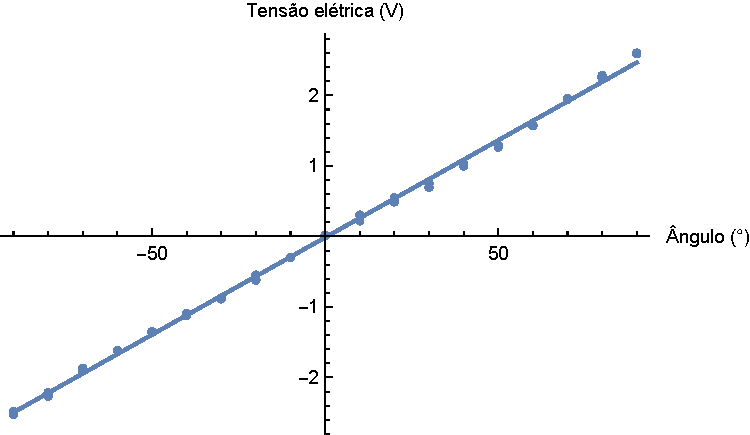
\includegraphics[width=0.8\textwidth]{Pendulo-fit.pdf}
\caption{Gráfico exibindo a função de transferência ajustada sobreposta às medidas experimentais}
\label{fig:pendulo-tf-sem-cond}
\end{figure}

\subsection{Função de transferência com condicionamento}

Na Tabela \ref{tab:pendulo-calibracao-condicionado}, estão apresentados os dados experimentais medidos utilizando o circuito de condicionamento:

\begin{table}[H]
\centering
\caption{Tabela da relação entre temperatura e a tensão elétrica medida com condicionamento}
\begin{tabular}{|l|l|l|}
 \hline
 \textbf{Ângulo ($º$)} & \textbf{Tensão Elétrica ($V$)} & \textbf{Tensão Elétrica ($V$)} \\ \hline

 -90 & -2.61 & -2.57 	\\ \hline
 -80 & -2.27 & -2.21 	\\ \hline
 -70 & -1.98 & -1.89 	\\ \hline
 -60 & -1.58 & -1.57 	\\ \hline
 -50 & -1.34 & -1.37 	\\ \hline
 -40 & -1.05 & -1.06 	\\ \hline
 -30 & -0.82 & -0.81 	\\ \hline
 -20 & -0.54 & -0.57 	\\ \hline
 -10 & 0.24 & 0.25 		\\ \hline
 0 & 0.50 & 0.70 		\\ \hline
 10 & 0.37 & 0.32 		\\ \hline
 20 & 0.62 & 0.58 		\\ \hline
 30 & 0.86 & 0.85 		\\ \hline
 40 & 1.21 & 1.12 		\\ \hline
 50 & 1.47 & 1.39 		\\ \hline
 60 & 1.82 & 1.70 		\\ \hline
 70 & 2.16 & 2.18 		\\ \hline
 80 & 2.51 & 2.44 		\\ \hline
 90 & 2.91 & 2.78 		\\ \hline

\end{tabular}
\label{tab:pendulo-calibracao-condicionado}
\end{table}

A função de transferência que melhor se ajusta aos dados experimentais da Tabela \ref{tab:pendulo-calibracao-condicionado} é dada pela equação \ref{eq:pendulo-tf-com-cond}:

\begin{equation}
	V(\theta) = 0.029 \theta + 0.125
	\label{eq:pendulo-tf-com-cond}
\end{equation}

\noindent 
ou em sua forma inversa, dada pela equação \ref{eq:pendulo-tf-com-cond-inv}:

\begin{equation}
	\theta(V) = -4.3 + 34. V
	\label{eq:pendulo-tf-com-cond-inv}
\end{equation}

O ajuste de curvas foi realizado com erro de linearidade dado conforme a Equação \ref{eq:pendulo-com-cond-rsquared}.

\begin{equation}
	R^2 = 0.989
	\label{eq:pendulo-com-cond-rsquared}
\end{equation}

De forma gráfica, os pontos medidos (Tabela \ref{tab:pendulo-calibracao-condicionado}) e a função de transferência (Equação \ref{eq:pendulo-tf-com-cond}) ajustada pode ser visualizada na figura \ref{fig:pendulo-tf-com-cond}.

\begin{figure}[H]
\centering
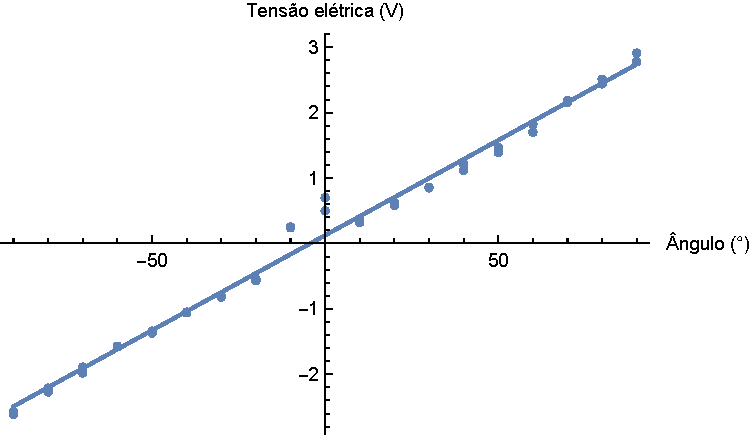
\includegraphics[width=0.8\textwidth]{Pendulo-Condicionado-fit.pdf}
\caption{Gráfico exibindo a função de transferência ajustada sobreposta às medidas experimentais}
\label{fig:pendulo-tf-com-cond}
\end{figure}

\subsection{Curva temporal do pêndulo}

A fim de obter uma curva de tensão elétrica em função do tempo, foi desenvolvido uma aplicação no LabVIEW que fosse capaz de exibir a curva extraída em tempo real na tela e pudesse exportar estes dados de forma que pudessem ser processados externamente. Na figura \ref{fig:pendulo-LabVIEW} está mostrado uma imagem do programa utilizado.

\begin{figure}[H]
\centering
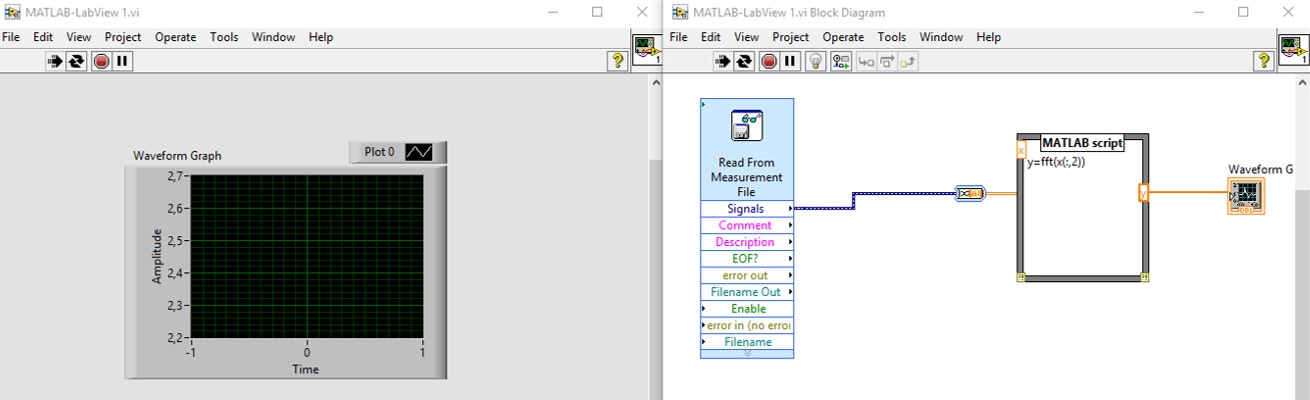
\includegraphics[width=\textwidth]{Imagens/labview_pendulo1.jpg}
\caption{Interface do LabVIEW para aquisição dos dados de tensão elétrica do pêndulo}
\label{fig:pendulo-LabVIEW}
\end{figure}

Após realizar a exportação dos dados foi utilizado o software MATLAB para importar estes dados em formato TSV (tab-separated values) e realizar o processamento. Primei- ramente, é importante notar que a informação importada está em valores de tensão elétrica (Volt) e tempo (segundo). Num primeiro passe, deseja-se filtrar o valor de forma a remover qualquer ruído gerado pelo conversor analógico-digital da placa de aquisição de dados e, após a filtragem, converter estes valores de tensão elétrica em uma posição angular utilizando a função de transferência inversa com condicionamento dada pela Equação \ref{eq:pendulo-tf-com-cond-inv}.

A figura \ref{fig:pendulo-curva-tensao-vs-tempo} apresenta a curva em forma bruta extraída diretamente do LabVIEW:

\begin{figure}[H]
\centering
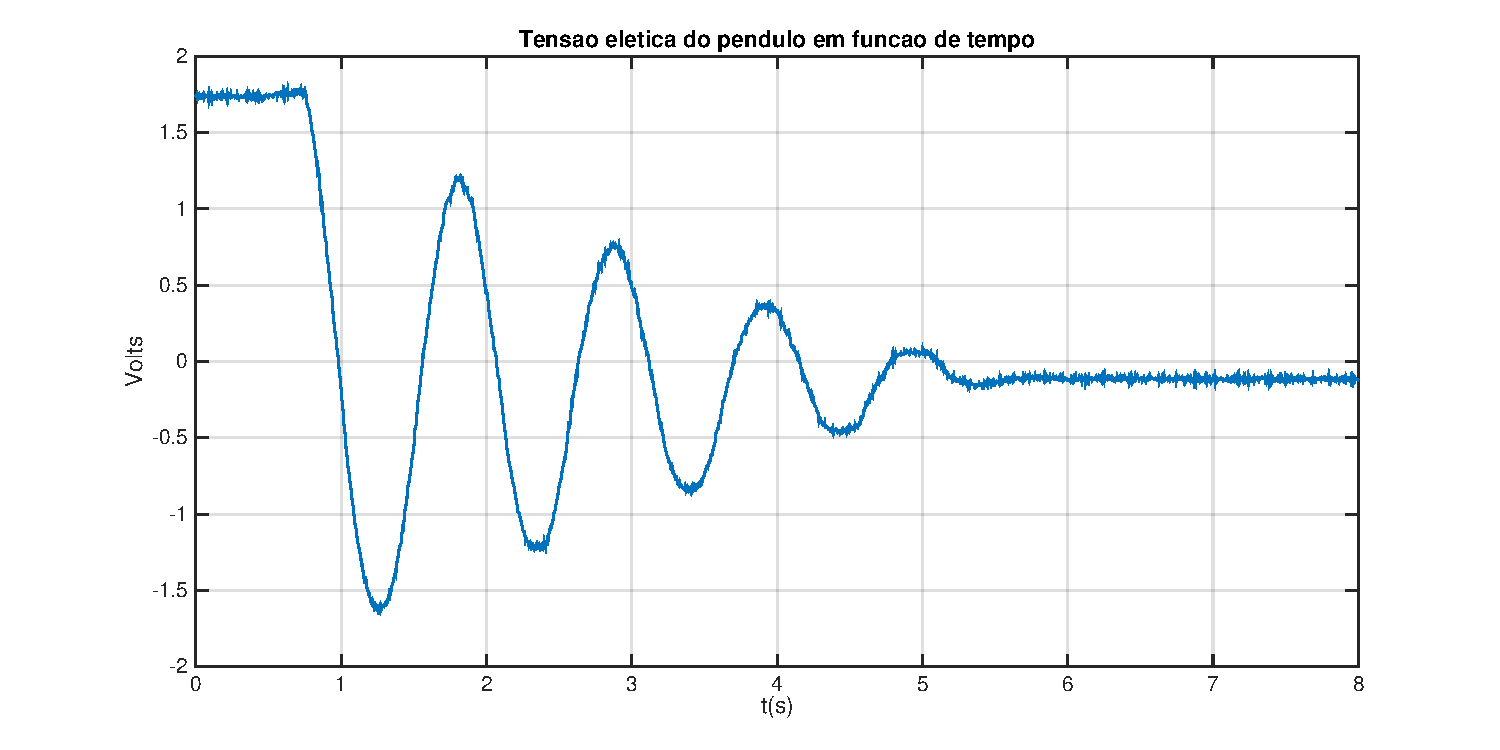
\includegraphics[width=\textwidth]{time-plot-raw.pdf}
\caption{Curva da tensão elétrica medida no pêndulo em função do tempo}
\label{fig:pendulo-curva-tensao-vs-tempo}
\end{figure}

Na curva \ref{fig:pendulo-curva-tensao-vs-tempo}, é possível observar que há um alto nível de ruído em alta frequência, isto é, frequências onde a frequência do ruído são de ordens muito superiores à frequência do sinal desejado. Dessa forma, um filtro passa baixas de Butterworth foi desenvolvido com frequência de corte em 20 $Hz$, que torna possível a extração da curva filtrada apresentada na figura \ref{fig:pendulo-curva-tensao-vs-tempo-filtrado}.

\begin{figure}[H]
\centering
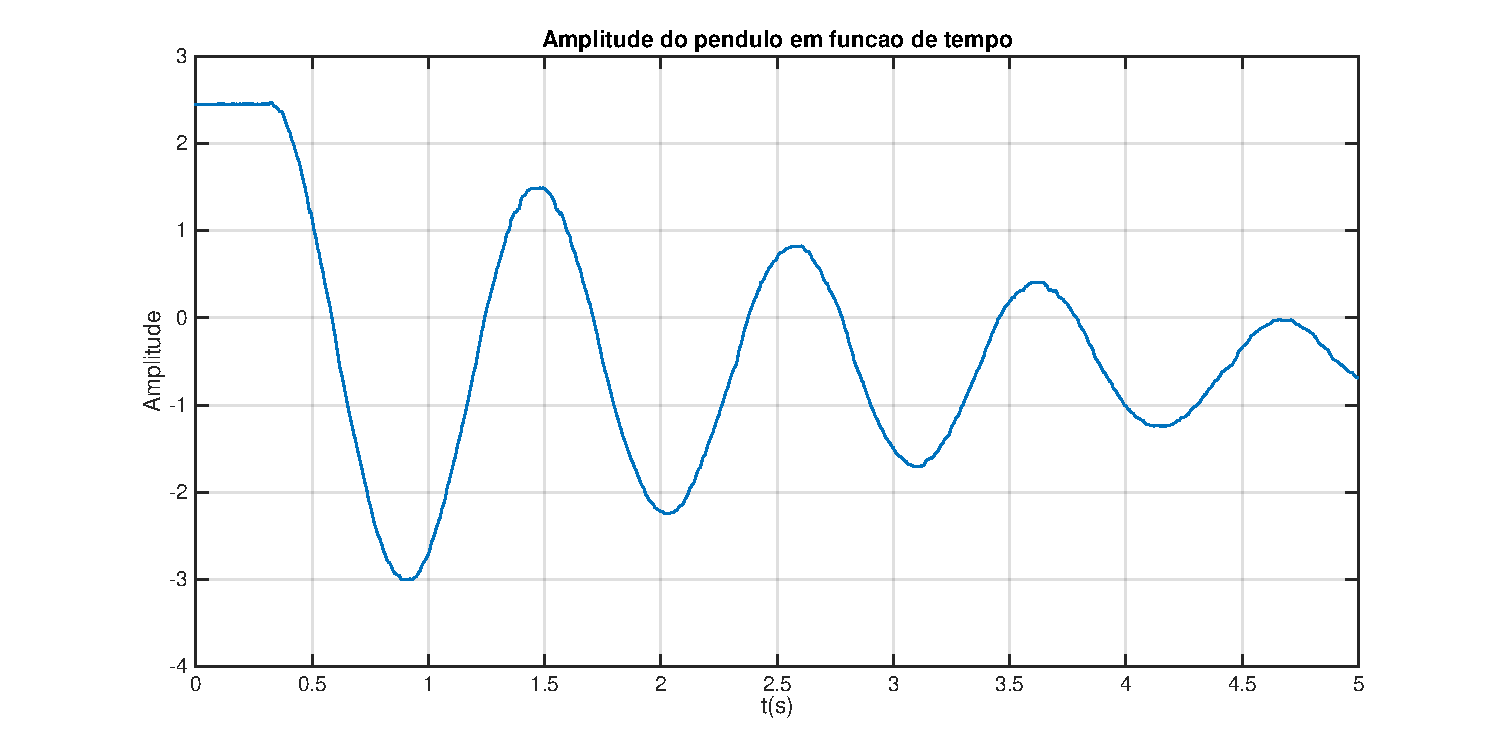
\includegraphics[width=\textwidth]{time-plot.pdf}
\caption{Curva da tensão elétrica medida no pêndulo em função do tempo, com filtro aplicado}
\label{fig:pendulo-curva-tensao-vs-tempo-filtrado}
\end{figure}

Uma vez que o ângulo de oscilação do pêndulo, quando conectado ao circuito de condicionamento, é dado pela equação \ref{eq:pendulo-tf-com-cond-inv}, é possível aplicar esta equação a cada um dos valores de tensão elétrica amostrados e converter esta curva em uma curva de posição angular em função do tempo. O resultado desta transformação está na figura \ref{fig:pendulo-curva-angulo-vs-tempo}. 

\begin{figure}[H]
\centering
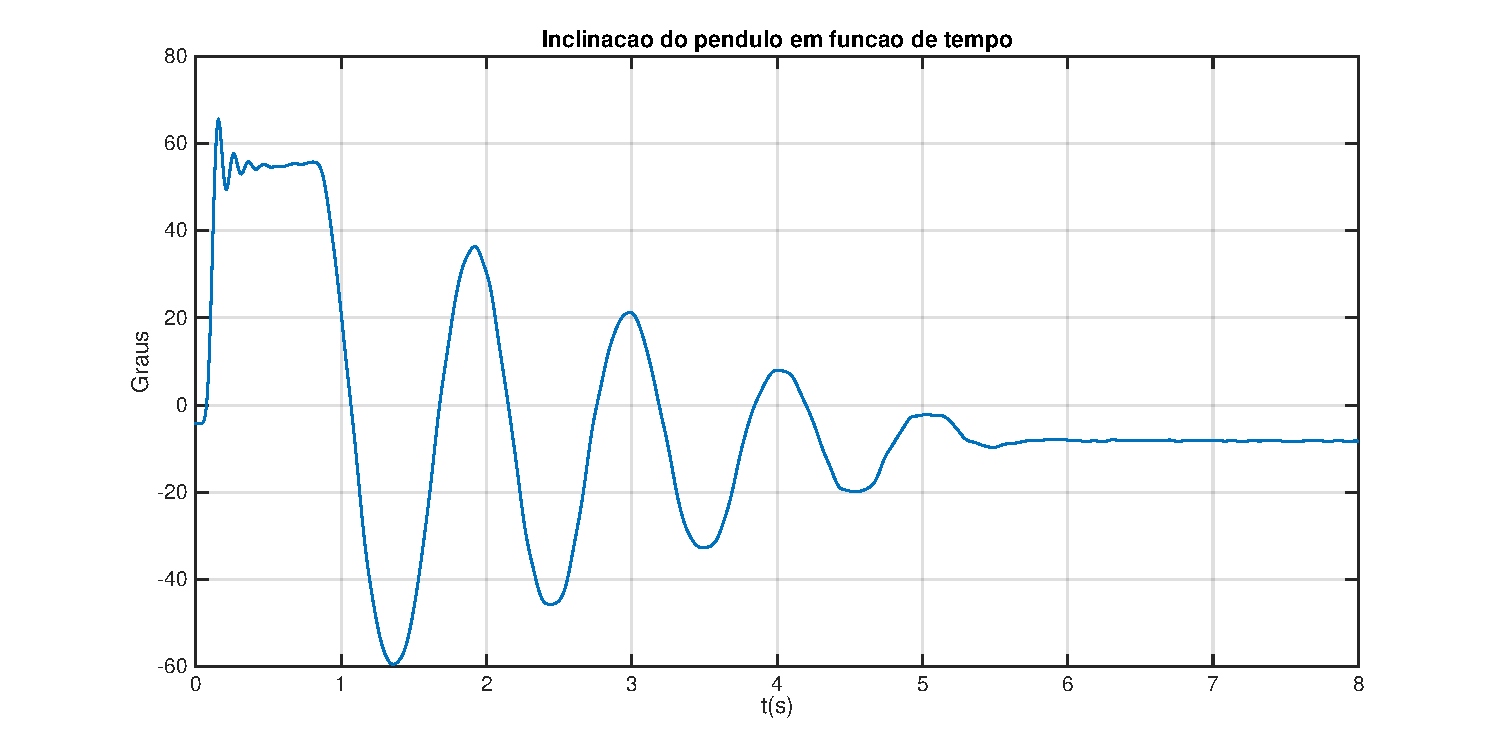
\includegraphics[width=\textwidth]{angle-time-plot.pdf}
\caption{Curva da posição angular do pêndulo em função do tempo}
\label{fig:pendulo-curva-angulo-vs-tempo}
\end{figure}

Adicionalmente, é possível calcular as componentes de frequência do sinal utilizando o algoritmo de \textit{Fast Fourier Transform} (FFT). Na figura \ref{fig:pendulo-frequencia} está apresentado a magnitude do espetro do sinal obtido.

\begin{figure}[H]
\centering
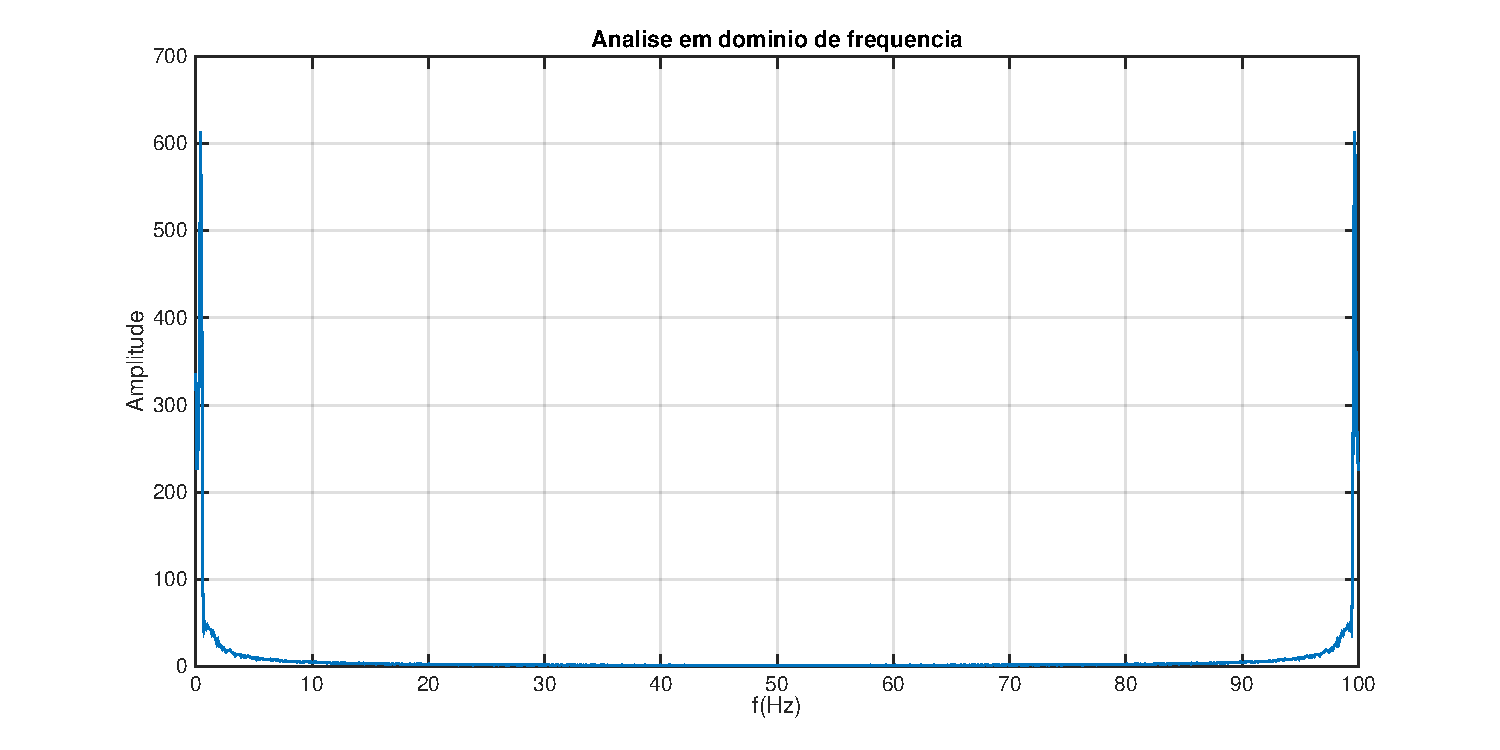
\includegraphics[width=\textwidth]{frequency-plot.pdf}
\caption{Análise de frequência da curva do pêndulo}
\label{fig:pendulo-frequencia}
\end{figure}

Para melhor visualizar o espectro, pode-se truncar o gráfico da imagem \ref{fig:pendulo-frequencia} em 1.5 $Hz$ para melhor visualizar a curva em baixa frequência, conforme figura \ref{fig:pendulo-frequencia-truncado}.

\begin{figure}[H]
\centering
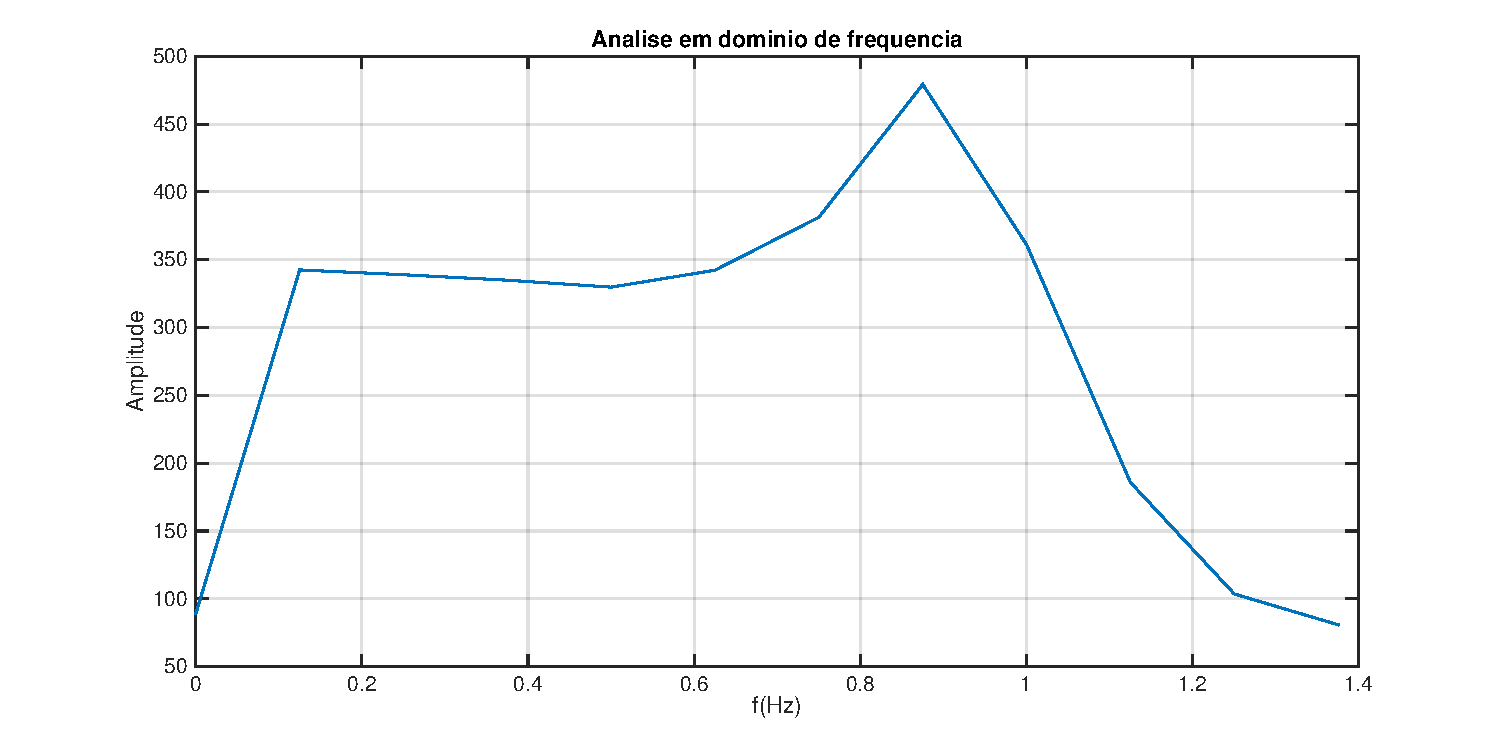
\includegraphics[width=\textwidth]{frequency-plot-slice.pdf}
\caption{Análise de frequência da curva do pêndulo (truncado em 1.5 $Hz$)}
\label{fig:pendulo-frequencia-truncado}
\end{figure}

Na figura \ref{fig:pendulo-frequencia-truncado}, é possível observar a componente espectral de $0.9$ $Hz$ no pêndulo. Esta componente também é claramente visível na curva temporal da figura \ref{fig:pendulo-curva-tensao-vs-tempo} onde o período da oscilação é de $1.1$ segundos, que correspondem ao valor de $0.9$ $Hz$.

As demais componentes contidas entre $0.1 Hz$ e $0.8 Hz$ são responsáveis pelo efeito de amortecimento do pêndulo, 

\subsection{Medição a 3 fios}

Considerando a ponte de \textit{Wheatstone} da figura \ref{fig:3fios-wheatstone}

\begin{figure}[H]
\centering
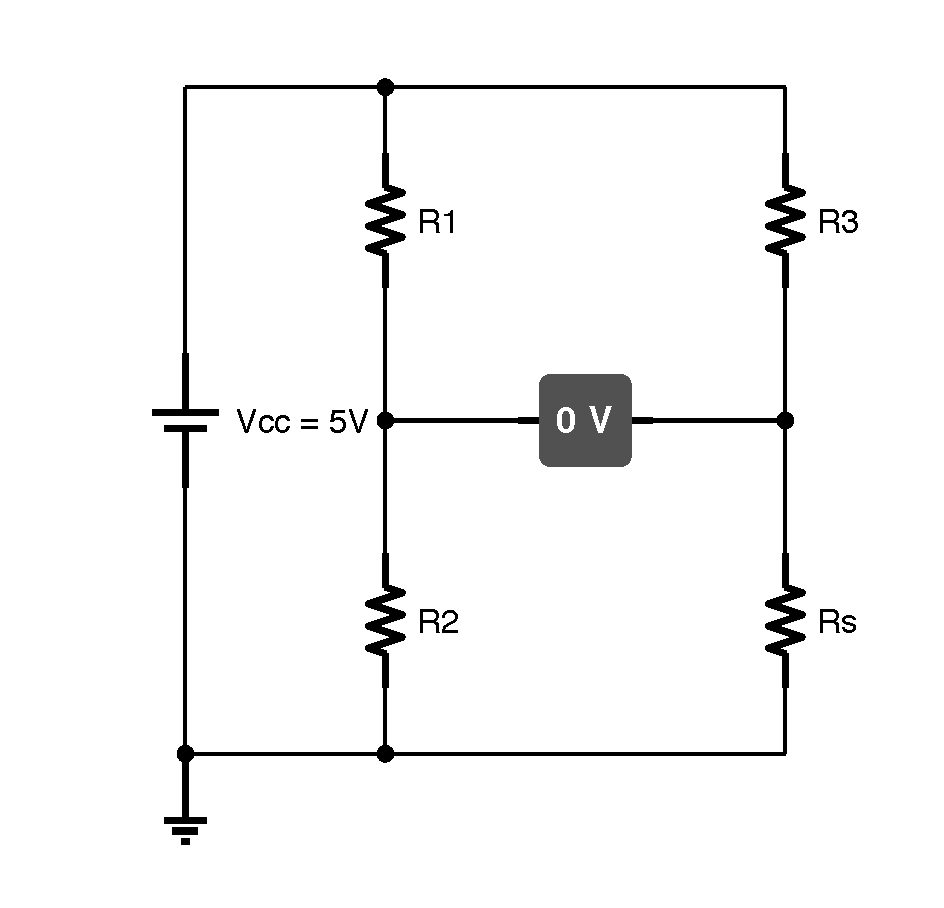
\includegraphics[width=0.6\textwidth]{Wheatstone-Bridge.pdf}
\caption{Ponte de Wheatstone equilibrada}
\label{fig:3fios-wheatstone}
\end{figure}

\noindent onde os resistores $R_1$, $R_2$ e $R_3$ são resistores fixos e definidos em função do valor de resistência máxima do sensor, $R_s$ é a resistência elétrica do sensor, variável em função da grandeza a ser medida, $V_{cc}$ é a tensão elétrica de alimentação da fonte e $V_o$ é a tensão elétrica de saída da ponte. É fácil provar que a equação correspondente ao circuito é dado pela equação \ref{eq:wheatstone-vo}:

\begin{equation}
	V_o = \left({{R_2}\over{R_1 + R_2}} - {{R_x}\over{R_x + R_3}}\right)V_{cc}
	\label{eq:wheatstone-vo}
\end{equation}

A ponte de Wheatstone pode ser vista como um circuito capaz de medir e aumentar pequenas diferenças de resistência elétrica de um sensor arbitrário em uma saída de tensão, com sensibilidade maior que a sensibilidade do sensor. Isto é, para uma pequena variação, é possível obter (com uma ponte devidamente projetada) uma saída em tensão elétrica com maior sensibilidade, quando comparada ao sensor isolado.

Embora esta característica seja ideal para utilizar em sensores cuja amplitude de variação de resistência elétrica seja muito pequena, isto também significa que não é possível desprezar as resistências elétricas intrínsecas dos fios de conexão do sensor com a ponte. Como a ponte de Wheatstone pode ser utilizada como um condicionador para pequenas variações de resistência elétrica, uma pequena inserção de resistência elétrica do fio pode causar um \textit{bias} significante na saída da ponte.

Com a finalidade de compensar esta não idealidade, é possível realizar medidas utilizando técnicas denominadas de \textbf{medida a 3 fios} e \textbf{medida a 4 fios}.

Nestas técnicas, um fio com as mesmas especificações de comprimento, seção reta e material é utilizado com a finalidade de tentar obter uma resistência elétrica semelhante ao fio de conexão do sensor e minimizar a significância do fio na medida. Este método pode ser expresso pelo seguinte circuito elétrico equivalente da figura \ref{fig:wheatstone-wire-model}:

\begin{figure}[H]
\centering
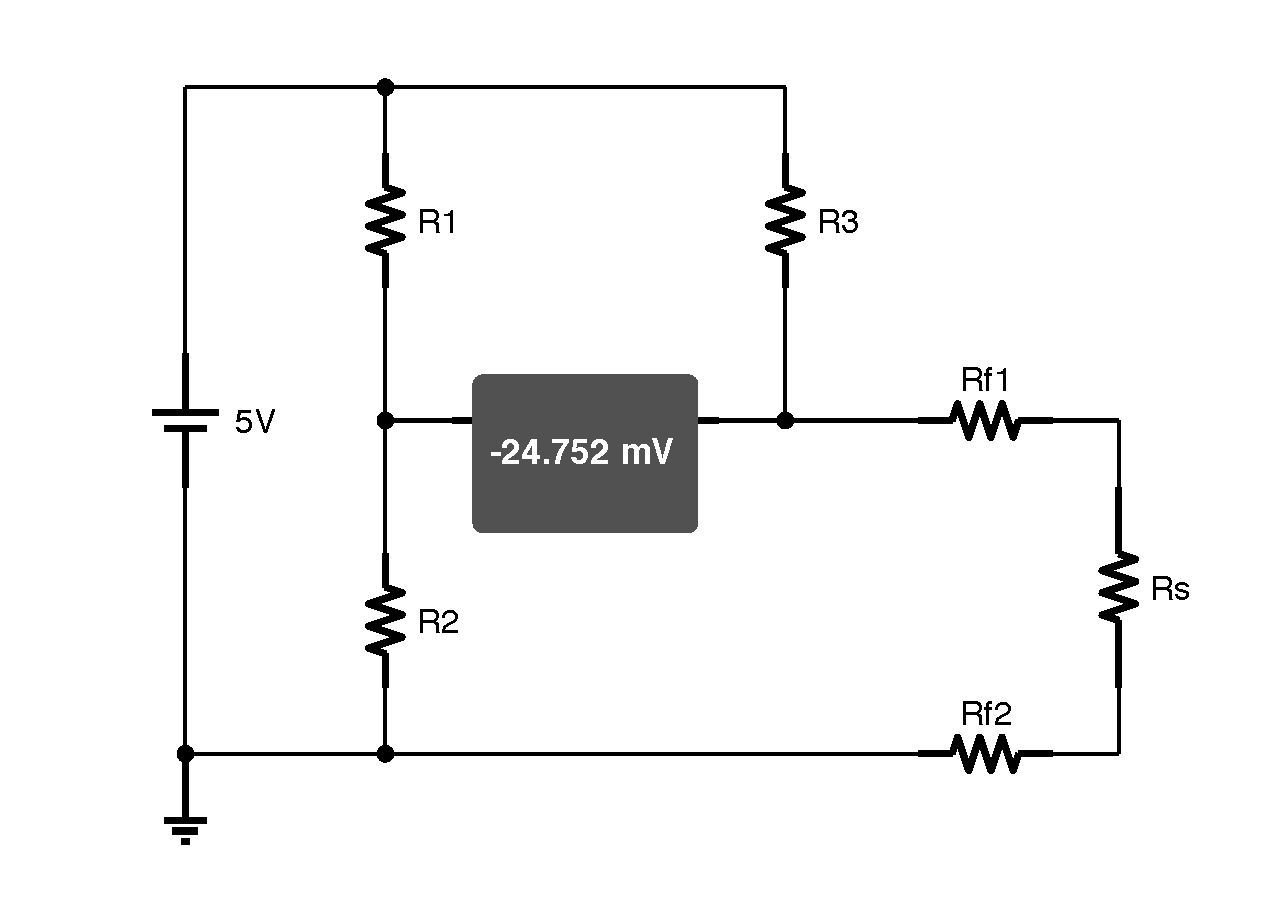
\includegraphics[width=0.6\textwidth]{Wheatstone-Bridge-WiresModel.pdf}
\caption{Ponte de Wheatstone com a resistência elétrica dos fios}
\label{fig:wheatstone-wire-model}
\end{figure}

\noindent onde os resistores $R_1$, $R_2$ e $R_3$ são resistores fixos e definidos em função do valor de resistência máxima do sensor, $R_s$ é a resistência elétrica do sensor, variável em função da grandeza a ser medida, $V_{cc}$ é a tensão elétrica de alimentação da fonte e o resistores $R_{fi}$ são resistências intrínsecas dos fios e espera-se que para fios de mesmo material, comprimento e seção reta, seus valores sejam semelhantes.

Conforme observa-se na figura \ref{fig:wheatstone-wire-model}, para os mesmos valores de $R_1$, $R_2$, $R_3$ e $R_f$ o valor de tensão elétrica de saída da ponte é diferente de zero. Isto é causado devido ao desbalanceamento da ponte causado pela resistência elétrica dos fios de conexão do sensor, representados por $R_{f1}$ e $R_{f2}$. Caso o sensor tenha uma variação pequena de resistência elétrica, o \textit{bias} causado pelas resistências série pode ser muito significante e gerar erros. Para reduzir o impacto dessa resistência série, pode-se utilizar o método de medida a 3 fios, onde um terceiro fio é conectado diretamente entre o sensor e um dos terminais do voltímetro, conforme figura \ref{fig:wheatstone-3wire}.

\begin{figure}[H]
\centering
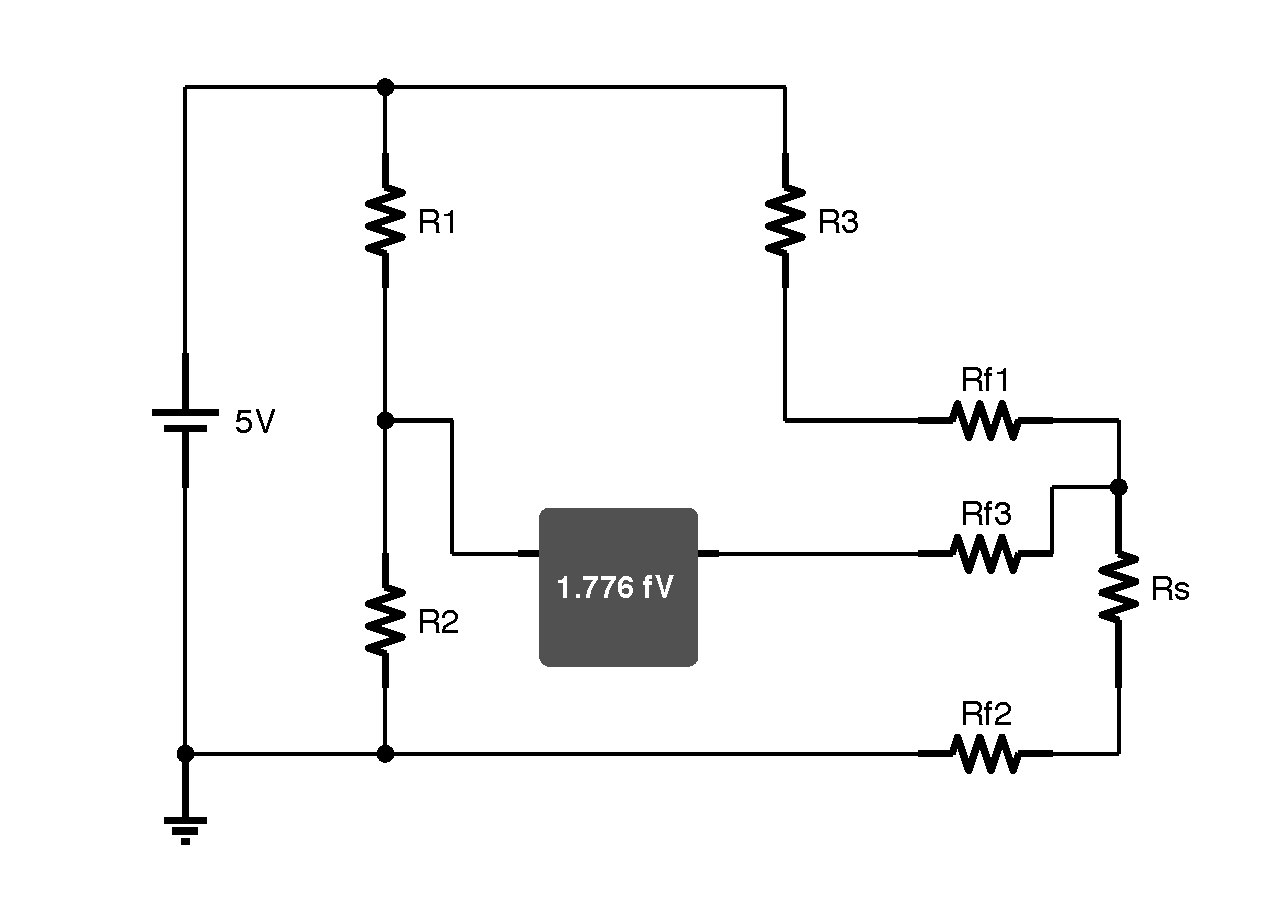
\includegraphics[width=0.6\textwidth]{Wheatstone-Bridge-3Wire.pdf}
\caption{Ponte de Wheatstone com medida a 3 fios}
\label{fig:wheatstone-3wire}
\end{figure}

\noindent onde foi adicionado um terceiro fio representado pela resistência $R_{f3}$ que representa a resistência elétrica do fio de conexão direta entre o voltímetro e o sensor. Nota-se que, para que o método seja eficaz, é necessário que o voltímetro tenha uma impedância elétrica muito alta a fim de evitar que haja uma queda de tensão elétrica sobre o resistor $R_{f3}$.

É possível observar claramente no resultado da simulação que o \textit{bias} produzido por esta construção ficou em $1.776 fV$, que dada a sensibilidade de um multímetro comercial de baixo custo, é imperceptível e a incerteza é no mínimo 1000 vezes superior (na ordem de mV).

\todo{equacionar isso}

\subsection{Medição a 4 fios}

Embora o método a 3 fios melhore bastante a qualidade da medida, há um offset dependente de $R_{f2}$ que considerando o comprimento do fio pode ser significante e afetar o resultado para sensores com baixas resistências elétricas associado com pequenas variações. Para solucionar este problema, há um outro método de medida que utiliza 4 fios e 2 instrumentos para realizar a medida com maior precisão, este método é denominado de \textbf{método a 4 fios}. Nele, é associado um amperímetro em série com o sensor e um voltímetro em paralelo com o mesmo e através de lei de Ohm, pode-se extrair o valor de resistência do sensor. Na figura \ref{fig:4wire-circuit} está apresentado o esquemático elético equivalente deste método.

\begin{figure}[H]
\centering
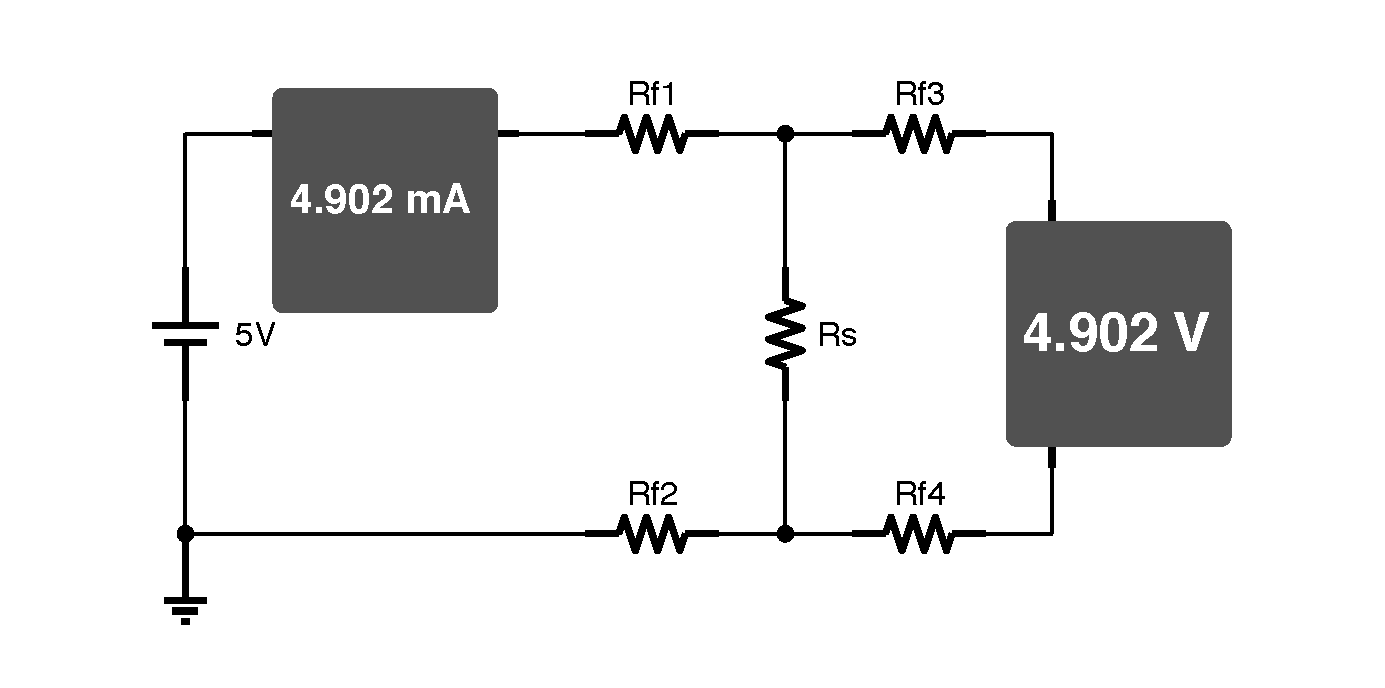
\includegraphics[width=0.6\textwidth]{4WireMeasure.pdf}
\caption{Esquemático elétrico do método de medida a 4 fios}
\label{fig:4wire-circuit}
\end{figure}

onde $R_s$ é a resistência elétrica do sensor e $R_f$ são as resistências elétricas dos fios de conexão do sensor e dos instrumentos.

Neste método, aplica-se diretamente a lei de Ohm conforme a equação \ref{eq:ohm}:

\begin{equation}
	R_s = \frac{V_s}{I_s}
	\label{eq:ohm}
\end{equation}

Independente da resistência elétrica dos fios, considerando que a impedância do voltímetro seja infinita ou muito grande, a queda de tensão provocada por $R_{f3}$ e $R_{f4}$ são negligenciáveis e a tensão medida sobre $R_s$ é a tensão real (respeitando a incerteza do instrumento). Para as resistências $R_{f1}$ e $R_{f2}$ a corrente elétrica que circula por elas é a mesma que circula por $R_s$, embora elas provoquem uma redução da corrente elétrica que circula pelo ramo, este é compensado na redução de tensão medida $V_s$. Logo, considerando-se somente o erro devido as conexões, o erro causado por esta construção é zero ou negligenciável.

%%%%%%%%%%%%%%%%%%%%%%%%%%%%%%%%%%%%%%%%%%%%%%%%%%%%%%%%%%%%%%%%%%%%%%%%%%%%%%

\todo{sensibilidade, resolução de entrada, resolução de saída, erro de linearidade ou de conformidade, incerteza, etc, assim como, a correspondente Cadeia de Medidas Proposta (teórica) e a Cadeia de Medidas Experimental}

\todo{LabVIEW+matlab}
\todo{só matlab}

\todo{determinar a sensibilidade, a resolução de entrada, resolução de saída, o erro de linearidade (ou erro de conformidade se for o caso) de seu sistema}

\todo{Tarefa para Casa: de posse da função de medição de seu sistema determinar a incerteza combinada deste sistema.}

\todo{com os sinais armazenados pelo programa LabVIEW elaborar um procedimento para determinar o decaimento em função do tempo e discutir esse resultado.}

\todo{Medição da Amplitude.}
\todo{Medição de $\theta_0$}
\todo{incertezas dos itens anteriores e dos comprimentos}

\todo{amortecimento}

\todo{medição do periodo}
\todo{grafico de amplitude e periodo}

\todo{modelo de thevenin}
\todo{grafico saida do pot vs angulo. qual erro?}
\todo{sensibilidade do circuito anterior}

\todo{discutir quantidade de amostras (medidas obtidas) para cada ângulo versus tensão.}
\todo{calcular a incerteza de TODAS medidas}

\section{Sensor de Efeito Hall Linear}
\todo{experimento do efeito hall}

\section{Módulo Sensor LED}
\todo{experimento do led}



\chapter{Conclusões}

\iftoggle{attachments}{
	\chapter*{Anexos}
	\section{Mathematica}
	\includenotebook{../Resources/Mathematica/Experimento 1-1.pdf}{Experimento 1}

	\section{LabVIEW}

	\section{MATLAB}
	\lstinputlisting[
		language=MATLAB,
		numbers=left,
		caption={Script MATLAB para análise de frequência}
	]{../Resources/MATLAB/primeiro.m}
}

\begin{thebibliography}{9}
\bibitem{mathematica-numerial-precision} \url{https://reference.wolfram.com/language/tutorial/NumericalPrecision.html}, acessado em 16 de março de 2016

%\bibitem{ref1} Sobrenome, A.B.; Sobrenome, C.D. Title of the cited article. Journal Title 2007, 6, 100-110. 
%\bibitem{ref2} Balbinot, A.; Brusamarello, V.J.. Title of the cited article. Journal Title 2007, 6, 100-110. 
%\bibitem{ref3} Author, A.; Author, B. Title of the chapter. In Book Title, 2nd ed.; Editor, A., Editor, B., Eds.; Publisher: Publisher Location, Country, 2007; Volume 3, pp. 154-196.
%\bibitem{ref4} Author, A.; Author, B. Book Title, 3rd ed.; Publisher: Publisher Location, Country, 2008; 
%pp. 154-196.

\todo{formatar essas referencias da forma correta... nao sei como ele quer}
\bibitem{datasheet-lm7805} Datasheet oferecido pelo fabricante do regulador de tensão LM7805
\bibitem{datasheet-lm7905} Datasheet oferecido pelo fabricante do regulador de tensão LM7905
\bibitem{datasheet-lm741} Datasheet oferecido pelo fabricante do amplificador operacional LM741

\todo{arrumar bibliografia}

\end{thebibliography}

\end{document}
